\documentclass{article}
\usepackage{gvv-book}
\usepackage{gvv}
\usepackage{amsmath}
\usepackage{amsfonts}
\usepackage{tikz}
\usepackage{setspace}
\usepackage{gensymb}
\usepackage[cmex10]{amsmath}
\usepackage{amsthm}
\usepackage{mathrsfs}
\usepackage{txfonts}
\usepackage{stfloats}
\usepackage{bm}
\usepackage{cite}
\usepackage{cases}
\usepackage{subfig}
\usepackage{longtable}
\usepackage{multirow}
\usepackage{enumitem}
\usepackage{mathtools}
\usepackage{tikz}
\usepackage{circuitikz}
\usepackage{verbatim}
\usepackage[breaklinks=true]{hyperref}
\usepackage{tkz-euclide}
\usepackage{listings}
\usepackage{color}    
\usepackage{array}    
\usepackage{longtable}
\usepackage{calc}     
\usepackage{multirow} 
\usepackage{hhline}   
\usepackage{ifthen}   
\usepackage{lscape}     
\usepackage{chngcntr}
\usepackage{graphicx}
\usepackage{float}
\usepackage{multicol}
\usepackage[a4paper, left = 1.5cm, right = 1.5cm]{geometry}


\begin{document}
\begin{center}
\large
    \textbf{ASSIGNMENT 2: GATE 2011 \\ AE : AEROSPACE ENGINEERING}\\
    AI25BTECH11029 - Samyak Gondane
\end{center}



\textbf{Read the following instructions carefully}

\begin{enumerate}
    \item Questions must be answered using computers provided by the GATE at the examination centers. Each computer shall run specialized examination software that permits a maximum of one answer to be selected for questions of multiple choice type.    
    \item Your answers shall be updated and saved on the server periodically and at the end of the examination. The examination will automatically stop once the duration of the examination is over.
    \item There are a total of \textbf{65} questions carrying 100 marks. All questions are of objective type.    
    \item Questions Q.1 – Q.25 carry 1-mark each, and questions Q.26 – Q.55 carry 2-marks each.    
    \item Questions Q.26 - Q.30 are of numerical answer type. For each of these questions, the correct answer is a number. All other questions are of multiple choice type. Each of these questions carries four choices for the answer labeled A, B, C and D. Only one of the four choices is the correct answer.    
    \item Questions Q.48 – Q.51 (2 pairs) are common data questions and question pairs (Q.52, Q.53) and (Q.54, Q.55) are linked answer questions. The answer to the second question of the linked answer questions depends on the answer to the first question of the pair. If the first question in the linked pair is wrongly answered or is unattempted, then the answer to the second question in the pair will not be evaluated.    
    \item Questions Q.56 – Q.65 belong to General Aptitude (GA). Questions Q.56 – Q.60 carry 1-mark each, and questions Q.61 – Q.65 carry 2-marks each.    
    \item Unattempted questions will result in zero mark. There is no negative marking for questions of numerical answer type, i.e., for Q.26 – Q.30. For questions of multiple choice type, wrong answers will result in \textbf{NEGATIVE} marks. For Q.1 – Q.25 and Q.56 – Q.60, $\frac{1}{3}$ mark will be deducted for each wrong answer. For Q.31 – Q.51 and Q.61 – Q.65, $\frac{2}{3}$ mark will be deducted for each wrong answer. The question pairs (Q.52, Q.53), and (Q.54, Q.55) are questions with linked answers. There will be negative marks only for wrong answer to the first question of the linked answer question pair, i.e. for Q.52 and Q.54, $\frac{2}{3}$ mark will be deducted for each wrong answer. There is no negative marking for Q.53 and Q.55.    
    \item Calculator is allowed whereas charts, graph sheets or tables are \textbf{NOT} allowed in the examination hall.    
    \item Rough work can be done in the specified area only.
    \item Candidates may use the back side of this page to record their answers for their own convenience.    
    \item To login, type your Registration Number and password as per instructions provided in the envelope.   
    \item In order to answer a question, you may select the question using the left side selection panel on the screen and choose the correct answer by clicking on the radio button next to the answer. The answered questions shall be indicated by a solid black ball on the selection panel. In order to change the answer, you may just click on another option. If you wish to leave a previously answered question unanswered, you may click on DESELECT ANSWER button.    
    \item You may also select questions using NEXT and PREVIOUS buttons.    
    \item You may also mark questions for reviewing later using MARK button. All marked questions are indicated by a rectangle in the selection panel. Questions which are answered but are marked for the review are indicated by a solid black rectangle and questions which are not answered but are marked for the review are indicated by an outlined rectangle in the selection panel.    
    \item You must sign this sheet and leave it with the invigilators at the end of the examination.
    
\end{enumerate}
\newpage

\textbf{DECLARATION}\\
\textbf{I hereby declare that I have read and followed all the instructions given in this sheet.}

\begin{center}
\begin{tikzpicture}
  \draw[thick] (0,0) rectangle (\textwidth,-2.5);
  \node[anchor=west] at (0.3,-0.5) {\textbf{Paper Code: AE}};
  \node[anchor=west] at (4.5,-0.5) {\textbf{Registration No:} \underline{\hspace{2.5cm}}};
  \node[anchor=west] at (9.5,-0.5) {\textbf{Name:} \underline{\hspace{4cm}}};
  \node[anchor=east] at (\textwidth-0.3,-2.2) {\textbf{Signature}};
\end{tikzpicture}
\end{center}





\textbf{Q.1 -- Q.25 carry one mark each}

\begin{enumerate}

\item Consider $x,y,z$ to be right-handed Cartesian coordinates. A vector function is defined in this coordinate system as $\textbf{v} = 3x\textbf{i} + 3xy\textbf{j} - yz^2\textbf{k}$ where $\textbf{i}, \textbf{j}$ and $\textbf{k}$ are the unit vectors along $x,y,z$ axes, respectively. The curl of $\textbf{v}$ is given by
\begin{multicols}{4}
\begin{enumerate}
\item $z^2\textbf{i} - 3y\textbf{k}$
\item $z^2\textbf{j} + 3y\textbf{k}$
\item $z^2\textbf{i} + 3y\textbf{j}$
\item $-z^2\textbf{i} + 3y\textbf{k}$
\end{enumerate}
\end{multicols}

\item Which of the following functions is periodic?
\begin{multicols}{4}
\begin{enumerate}
\item $f(x) = x^2$
\item $f(x) = \log x$
\item $f(x) = e^x$
\item $f(x) = const.$
\end{enumerate}
\end{multicols}

\item The function $f(x_1,x_2,x_3)=x_1^2+x_2^2+x_3^2-4x_1-6x_2+14$ has its minimum value at
\begin{multicols}{4}
\begin{enumerate}
\item (1,2,3)
\item (0,0,0)
\item (3,2,1)
\item (1,1,3)
\end{enumerate}
\end{multicols}

\item Consider the function $f(x_1,x_2)=x_1^2+x_2^2+2x_1-2x_2+e^{-(x_1^2+x_2^2)}$. The vector pointing in the direction of maximum increase of the function at the point $(1,-1)$ is
\begin{multicols}{4}
\begin{enumerate}
\item $\begin{pmatrix}2\\-5\end{pmatrix}$
\item $\begin{pmatrix}1\\-5\end{pmatrix}$
\item $\begin{pmatrix}0.73\\-6.73\end{pmatrix}$
\item $\begin{pmatrix}2\\-4\end{pmatrix}$
\end{enumerate}
\end{multicols}

\item Two simultaneous equations given by $x+y=\pi$ and $x-y=-\pi$ have
\begin{multicols}{2}
\begin{enumerate}
\item a unique solution
\item infinitely many solutions
\item no solution
\item a finite number of multiple solutions
\end{enumerate}
\end{multicols}

\item In three-dimensional linear elastic solids, the number of non-trivial stress–strain relations, strain–displacement equations and equations of equilibrium are, respectively,
\begin{multicols}{4}
\begin{enumerate}
\item 3, 3 and 3
\item 6, 3 and 3
\item 6, 6 and 3
\item 6, 3 and 6
\end{enumerate}
\end{multicols}

\item An Euler–Bernoulli beam in bending is assumed to satisfy
\begin{enumerate}
\item both plane stress as well as plane strain conditions
\item plane strain condition but not plane stress condition
\item plane stress condition but not plane strain condition
\item neither plane strain condition nor plane stress condition
\end{enumerate}

\item A statically indeterminate frame structure has
\begin{enumerate}
\item same number of joint degrees of freedom as the number of equilibrium equations
\item number of joint degrees of freedom greater than the number of equilibrium equations
\item number of joint degrees of freedom less than the number of equilibrium equations
\item unknown number of joint degrees of freedom, which cannot be solved using laws of mechanics
\end{enumerate}

\item Consider a single degree of freedom spring-mass-damper system with mass $m$, damping $c$ and stiffness $k$. The logarithmic decrement of this system can be calculated using
\begin{multicols}{4}
\begin{enumerate}
\item $\frac{2\pi c}{\sqrt{4mk - c^2}}$
\item $\frac{\pi c}{\sqrt{4mk - c^2}}$
\item $\frac{2\pi c}{\sqrt{mk - c^2}}$
\item $\frac{2\pi c}{\sqrt{mk - 4c^2}}$
\end{enumerate}
\end{multicols}

\item Consider a single degree of freedom spring-mass system of spring stiffness $k_1$ and mass $m$ which has a natural frequency of $10$ rad/s. Consider another single degree of freedom spring-mass system of spring stiffness $k_2$ and mass $m$ which has a natural frequency of $20$ rad/s. The spring stiffness $k_2$ is equal to
\begin{multicols}{4}
\begin{enumerate}
\item $k_1$
\item $2k_1$
\item $\frac{k_1}{4}$
\item $4k_1$
\end{enumerate}
\end{multicols}

\item Consider a simply supported two-dimensional beam.
\begin{figure}[H]
    \centering
    \documentclass{}
\usepackage{}
\usetikzlibrary{shapes, arrows.meta}

\begin{document}

\begin{tikzpicture}[scale=0.5]

\draw[thick] (0,0) -- (6,0);

\draw[thick] (0,0) -- (-0.5,-0.5) -- (0.5,-0.5) -- cycle;
\draw[-{Latex}, thick] (-0.3,-0.5) -- (-0.3,-1); % vertical reaction

\draw[thick] (6,0) -- (5.5,-0.5) -- (6.5,-0.5) -- cycle;
\draw[thick] (5.7,-0.5) circle (0.2);
\draw[thick] (6.3,-0.5) circle (0.2);
\draw[-{Latex}, thick] (6.3,-0.7) -- (6.3,-1.2); % vertical reaction

\end{tikzpicture}

\end{document}
    \caption{}
    \label{fig:q11(1)}
\end{figure}
If the beam is converted into a fixed-fixed beam,
\begin{figure}[H]
        \centering
        \begin{figure}[!ht]
\centering
\resizebox{0.25\textwidth}{!}{%
\begin{circuitikz}
\tikzstyle{every node}=[font=\LARGE]
\draw [ line width=0.7pt](7,11.75) to[short] (13.25,11.75);
\draw (13.25,12.25) to[short] (13.25,11.25);
\draw (7,12.25) to[short] (7,11.25);
\draw (13.25,12.25) to[short] (13.75,12.75);
\draw (13.25,11.75) to[short] (13.75,12.25);
\draw (13.25,11.25) to[short] (13.75,11.75);
\draw (7,12.25) to[short] (6.5,11.75);
\draw (7,11.75) to[short] (6.5,11.25);
\draw (7,11.25) to[short] (6.5,10.75);
\end{circuitikz}
}%

\label{fig:my_label}
\end{figure}
        \caption{}
        \label{fig:q11(2)}
    \end{figure}
then the degree of static indeterminacy will
\begin{multicols}{4}
\begin{enumerate}
\item increase by 3
\item increase by 2
\item decrease by 1
\item decrease by 3
\end{enumerate}
\end{multicols}

\item An impulsive launch of a rocket minimizes the loss of burn-out velocity due to
\begin{enumerate}
\item aerodynamic drag force only
\item gravitational force only
\item both aerodynamic drag and gravitational forces
\item reaction jet control force
\end{enumerate}

\item Multi-staging in rockets improves the burn-out performance by increasing mainly stage-wise
\begin{multicols}{2}
\begin{enumerate}
\item payload mass ratios
\item structural mass efficiencies
\item propellant masses
\item control system masses
\end{enumerate}
\end{multicols}

\item In an un-powered glide of an aircraft having weight $W$, lift $L$ and drag $D$, the equilibrium glide angle is defined as
\begin{multicols}{4}
\begin{enumerate}
\item $\tan^{-1}(\frac{L}{D})$
\item $\tan^{-1}(\frac{D}{L})$
\item $\tan^{-1}(\frac{L}{W})$
\item $\tan^{-1}(\frac{W}{L})$
\end{enumerate}
\end{multicols}

\item Lift on an aircraft climbing vertically up is
\begin{multicols}{2}
\begin{enumerate}
\item equal to its weight
\item zero
\item equal to the drag
\item equal to the thrust
\end{enumerate}
\end{multicols}

\item If an aircraft is performing a positive yawing manoeuvre, the side slip angle
\begin{multicols}{4}
\begin{enumerate}
\item is always zero
\item is never zero
\item is always negative
\item could be any value
\end{enumerate}
\end{multicols}

\item For an airplane to be statically stable, its centre of gravity must always be
\begin{multicols}{2}
\begin{enumerate}
\item ahead of wing aerodynamic centre
\item aft of the wing aerodynamic centre
\item ahead of neutral point
\item aft of neutral point
\end{enumerate}
\end{multicols}

\item It is seen that the drag polar of a certain aerofoil is symmetric about the $C_d$ axis. This drag polar could refer to
\begin{multicols}{4}
\begin{enumerate}
\item NACA 0012
\item NACA 4415
\item NACA 23012
\item None of the above
\end{enumerate}
\end{multicols}

\item The aerodynamic centre of a supersonic aerofoil, with chord $c$, is located at
\begin{multicols}{4}
\begin{enumerate}
\item the leading edge
\item $0.25c$
\item $0.5c$
\item $0.75c$
\end{enumerate}
\end{multicols}

\item Winglets are used on wings to minimize
\begin{multicols}{4}
\begin{enumerate}
\item skin friction drag
\item profile drag
\item wave drag
\item induced drag
\end{enumerate}
\end{multicols}

\item Consider a potential flow with free stream velocity $V_\infty$, over a spinning circular cylinder of radius $R$ and circulation $\Gamma$. The stream function $\psi$, where $\psi=0$ on the cylinder surface, in cylindrical coordinates $(r,\theta)$ is given by
\begin{multicols}{2}
\begin{enumerate}
\item $V_\infty r \left(1-\frac{R^2}{r^2}\right)\cos\theta + \frac{\Gamma}{2\pi}\ln\frac{r}{R}$
\item $V_\infty r \left(1+\frac{R^2}{r^2}\right)\cos\theta + \frac{\Gamma}{2\pi}\ln\frac{r}{R}$
\item $V_\infty r \left(1-\frac{R^2}{r^2}\right)\sin\theta + \frac{\Gamma}{2\pi}\ln\frac{r}{R}$
\item $V_\infty r \left(1+\frac{R^2}{r^2}\right)\sin\theta + \frac{\Gamma}{2\pi}\ln\frac{r}{R}$
\end{enumerate}
\end{multicols}

\item A main objective of by-pass in a turbo-fan engine is to increase
\begin{multicols}{2}
\begin{enumerate}
\item mass flow rate through engine inlet
\item turbine inlet temperature
\item mass flow rate through exhaust nozzle
\item compressor pressure ratio
\end{enumerate}
\end{multicols}

\item The pressure ratio in any one stage of a jet engine compressor is limited by
\begin{enumerate}
\item entry stagnation temperature in that stage
\item entry Mach number in that stage
\item pressure-gradient-induced separation in that stage
\item mass flow rate in that stage
\end{enumerate}

\item Thermodynamic cycle on which the jet engine operates can be
\begin{multicols}{2}
\begin{enumerate}
\item open Rankine cycle only
\item either open or closed Rankine cycle
\item open Brayton cycle only
\item either open or closed Brayton cycle
\end{enumerate}
\end{multicols}

\item Propulsion efficiency of a jet engine is
\begin{enumerate}
\item directly proportional to both the thrust power and the air mass flow rate
\item inversely proportional to both the thrust power and the air mass flow rate
\item directly proportional to the thrust power and inversely proportional to the air mass flow rate
\item inversely proportional to the thrust power and directly proportional to the air mass flow rate
\end{enumerate}


\textbf{Q.26 -- Q.55 carry two marks each.}\\
\textbf{Questions Q.26 to Q.30 are numerical answer type. The answer to each of these questions is either a positive whole number, or a positive real number with maximum of 2 decimal places.}


\item Consider a cantilever beam having length $L=1\ m$, square cross-section (width = depth = 0.01 m) and Young’s modulus $50\ GPa$. The beam is subjected to a transverse load $P=1\ N$ at the mid-span ($L/2$) at the center of the cross-section. Under the small deformation theory, the transverse deflection of the beam (in mm) at its free-end is \underline{\hspace{2cm}}.
\begin{figure}[H]
    \centering
    \begin{center}
\renewcommand{\arraystretch}{1.35}
\setlength{\tabcolsep}{6pt}
\begin{tabular}{ |p{3.6cm}|p{4.4cm}|p{3.6cm}| }
  \hline
  {\centering \textbf{Age group of\\ mine workers}\par} &
  {\centering \textbf{Age-specific injury rate\\ (per 1000 persons)}\par} &
  {\centering \textbf{Age-specific population\\ in the mine}\par} \\
  \hline
  {\centering 18--32\par} & {\centering 1.8\par} & {\centering 1000\par} \\ \hline
  {\centering 33--46\par} & {\centering 2.5\par} & {\centering 500\par}  \\ \hline
  {\centering 47--60\par} & {\centering 4.5\par} & {\centering 300\par}  \\ \hline
\end{tabular}
\end{center}

    \caption{}
    \label{fig:q26}
\end{figure}

\item Consider a beam in bending with a solid circular cross-section of $1$ \text{mm}$^2$, which is subjected to a transverse shear force of $1$ N. The shear stress at the center of the cross-section (in N/mm$^2$) is \underline{\hspace{2cm}}.

\item A simply supported slender column of square cross section (width = depth = $d$) has to be designed such that it buckles at the same instant as it yields. Length of the column is $1.57$ m and it is made of a material whose Young’s modulus is $200$ GPa and yield stress is $240$ MPa. The width, $d$, of the column (in cm) should be \underline{\hspace{2cm}}.

\item A turbojet powered aircraft is flying at Mach number $0.8$ at an altitude of $10$ km. The inlet and exit areas of the engine are $0.7$ m$^2$ and $0.4$ m$^2$ respectively. The exhaust gases have velocity of $500$ m/s and pressure of $60$ kPa. The free stream pressure, density and speed of sound are $26.5$ kPa, $0.413$ kg/m$^3$ and $299.5$ m/s respectively. The thrust of the engine (in kN) is \underline{\hspace{2cm}}.

\item A low speed wind tunnel has a contraction ratio of 14:1 and the cross-sectional area of the test section is 1 m$^2$. The static pressure difference between the settling chamber and the test section is 40 cm of water column. Assume $g=9.81$ m/s$^2$, $\rho_{\text{air}}=1.2$ kg/m$^3$ and $\rho_{\text{water}}=1000$ kg/m$^3$. The speed of air in the test section (in m/s) is \underline{\hspace{2cm}}.
\\\\
\textbf{Questions Q.31 to Q.55 are multiple choice type.}

\item Consider the function $f(x)=x-\sin x$. The Newton–Raphson iteration formula to find the root of the function starting from an initial guess $x^{(0)}$ at iteration $k$ is
\begin{multicols}{2}
\begin{enumerate}
\item $x^{(k+1)}=\frac{\sin x^{(k)}- x^{(k)}\cos x^{(k)}}{1-\cos x^{(k)}}$
\item $x^{(k+1)}=\frac{\sin x^{(k)}- x^{(k)}\cos x^{(k)}}{1+\cos x^{(k)}}$
\item $x^{(k+1)}=\frac{\sin x^{(k)}+ x^{(k)}\cos x^{(k)}}{1-\cos x^{(k)}}$
\item $x^{(k+1)}=\frac{\sin x^{(k)}+ x^{(k)}\cos x^{(k)}}{1+\cos x^{(k)}}$
\end{enumerate}
\end{multicols}

\item Consider the matrix $\myvec{a & 2 \\ b & 2}$ where $a$ and $b$ are real numbers. The two eigenvalues of this matrix $\lambda_1$ and $\lambda_2$ are real and distinct $(\lambda_1\neq\lambda_2)$ when
\begin{multicols}{4}
\begin{enumerate}
\item $a>0$ and $b<0$
\item $a>0$ and $b>0$
\item $a<0$ and $b<0$
\item $a=0$ and $b=0$
\end{enumerate}
\end{multicols}

\item The solution of $\frac{dy}{dt}=y^3e^tt^2$ with initial condition $y(0)=1$ is given by
\begin{multicols}{2}
\begin{enumerate}
\item $\frac{1}{9}e^t(t+3)^2$
\item $\sqrt{\frac{9}{5 + 2e^t(t^2 - 2t + 2)}}$
\item $\frac{4e^t}{(t + 2)^2}$
\item $\sqrt{\frac{1}{5 - 2e^t(t^2 - 2t + 2)}}$
\end{enumerate}
\end{multicols}

\item A jet engine is operating at a Mach number of $0.8$ at an altitude of $10$ km. The efficiency of the air intake is $0.8$ and that of the compressor is $0.87$. The total temperatures (in K) at the exits of the air intake and the compressor respectively are (Ambient pressure $=26.5$ kPa; Ambient temperature $=223.3$ K; $\gamma=1.4$)
\begin{multicols}{4}
\begin{enumerate}
\item 251.9 and 458.2
\item 234.9 and 486.8
\item 251.9 and 486.8
\item 234.9 and 458.2
\end{enumerate}
\end{multicols}

\item A rocket engine is tested on a test bed under the ideal condition of fully expanded jet. The exhaust velocity is $2000$ m/s through a nozzle of area $2.5$ m$^2$. The mass flow rate is $200$ kg/s. The specific impulse of the propellant and the thrust developed respectively are (assume $g=9.81$ m/s$^2$)
\begin{multicols}{2}
\begin{enumerate}
\item $175.87\ s$ and $200\ kN$
\item $203.87\ s$ and $400\ kN$
\item $231.87\ s$ and $200\ kN$
\item $203.87\ s$ and $200\ kN$
\end{enumerate}
\end{multicols}

\item A body undergoes deformation under plane strain conditions when subjected to the following stresses (in MPa): $\sigma_{xx}=450,\ \sigma_{yy}=450,\ \tau_{xy}=75,\ \tau_{xz}=0,\ \tau_{yz}=0$. What are the remaining components of stresses (in MPa) and strains? Assume the material to be isotropic and linear-elastic with Young’s modulus $E=200$ GPa and Poisson’s ratio $\nu=1/3$.
\begin{enumerate}
\item $\sigma_{zz}=0, \ \epsilon_{xx}=0.00225,\ \epsilon_{yy}=0.00225,\ \gamma_{xy}=0.0020,\ \gamma_{xz}=0,\ \gamma_{yz}=0$
\item $\sigma_{zz}=300, \ \epsilon_{xx}=0.001,\ \epsilon_{yy}=0.001,\ \gamma_{xy}=0.001,\ \gamma_{xz}=0,\ \gamma_{yz}=0$
\item $\sigma_{zz}=300, \ \epsilon_{xx}=0.00225,\ \epsilon_{yy}=0.00225,\ \gamma_{xy}=0.001,\ \gamma_{xz}=0,\ \gamma_{yz}=0$
\item $\sigma_{zz}=0, \ \epsilon_{xx}=0.001,\ \epsilon_{yy}=0.001,\ \gamma_{xy}=0.002,\ \gamma_{xz}=0,\ \gamma_{yz}=0$
\end{enumerate}

\item Which of the following Airy’s stress functions could satisfy the given boundary conditions, assuming constant values of $\sigma_{xx}=P$, $\sigma_{yy}=Q$ and $\tau_{xy}=R$, along the boundary?
\begin{figure}[H]
    \centering
    \begin{figure}[!ht]
\centering
\resizebox{0.3\textwidth}{!}{%
\begin{circuitikz}
\tikzstyle{every node}=[font=\normalsize]
\draw [ line width=1.4pt ] (8.75,13.5) rectangle (15.5,10);
\draw [line width=0.9pt, ->, >=Stealth] (11.75,12) -- (11.75,12.75);
\draw [line width=0.9pt, ->, >=Stealth] (11.75,12) -- (13,12);
\node [font=\normalsize] at (11.5,12.75) {y};
\node [font=\normalsize] at (13.5,11.75) {x};
\draw [line width=0.9pt, ->, >=Stealth] (9,13.5) -- (9,14.25);
\draw [line width=0.9pt, ->, >=Stealth] (10,13.5) -- (10,14.25);
\draw [line width=0.9pt, ->, >=Stealth] (11,13.5) -- (11,14.25);
\draw [line width=0.9pt, ->, >=Stealth] (12,13.5) -- (12,14.25);
\draw [line width=0.9pt, ->, >=Stealth] (13,13.5) -- (13,14.25);
\draw [line width=0.9pt, ->, >=Stealth] (14,13.5) -- (14,14.25);
\draw [line width=0.9pt, ->, >=Stealth] (15,13.5) -- (15,14.25);
\draw [line width=0.9pt, ->, >=Stealth] (9,10) -- (9,9.25);
\draw [line width=0.9pt, ->, >=Stealth] (10,10) -- (10,9.25);
\draw [line width=0.9pt, ->, >=Stealth] (11.25,10) -- (11.25,9.25);
\draw [line width=0.9pt, ->, >=Stealth] (12.25,10) -- (12.25,9.25);
\draw [line width=0.9pt, ->, >=Stealth] (13.25,10) -- (13.25,9.25);
\draw [line width=0.9pt, ->, >=Stealth] (14.5,10) -- (14.5,9.25);
\draw [line width=0.9pt, ->, >=Stealth] (15.5,13.25) -- (16.25,13.25);
\draw [line width=0.9pt, ->, >=Stealth] (15.5,12.25) -- (16.5,12.25);
\draw [line width=0.9pt, ->, >=Stealth] (15.5,11) -- (16.5,11);
\draw [line width=0.9pt, ->, >=Stealth] (8.75,12.75) -- (8,12.75);
\draw [line width=0.9pt, ->, >=Stealth] (8.75,11.75) -- (8,11.75);
\draw [line width=0.9pt, ->, >=Stealth] (8.75,10.5) -- (8,10.5);
\draw [line width=0.9pt, ->, >=Stealth] (8.75,14) -- (9.5,14);
\draw [line width=0.9pt, ->, >=Stealth] (10.25,14) -- (11.25,14);
\draw [line width=0.9pt, ->, >=Stealth] (11.75,14) -- (12.5,14);
\draw [line width=0.9pt, ->, >=Stealth] (13,14) -- (13.75,14);
\draw [line width=0.9pt, ->, >=Stealth] (14.25,14) -- (15.25,14);
\draw [line width=0.9pt, ->, >=Stealth] (15.75,11.75) -- (15.75,12.75);
\draw [line width=0.9pt, ->, >=Stealth] (16,10.5) -- (16,11.5);
\draw [line width=0.9pt, ->, >=Stealth] (9.5,9.75) -- (8.5,9.75);
\draw [line width=0.9pt, ->, >=Stealth] (10.5,9.75) -- (9.75,9.75);
\draw [line width=0.9pt, ->, >=Stealth] (11.75,9.75) -- (11,9.75);
\draw [line width=0.9pt, ->, >=Stealth] (12.75,9.75) -- (12,9.75);
\draw [line width=0.9pt, ->, >=Stealth] (13.75,9.75) -- (13,9.75);
\draw [line width=0.9pt, ->, >=Stealth] (15,9.75) -- (14,9.75);
\draw [line width=0.9pt, ->, >=Stealth] (8.5,13.25) -- (8.5,12.25);
\draw [line width=0.9pt, ->, >=Stealth] (8.5,11.5) -- (8.5,10.5);
\end{circuitikz}
}%

\label{fig:my_label}
\end{figure}
    \caption{}
    \label{fig:q37}
\end{figure}
\begin{multicols}{2}
\begin{enumerate}
\item $\phi= \frac{P}{2}x^2 + \frac{Q}{2}y^2 - Rxy$
\item $\phi= \frac{P}{2}y^2 + \frac{Q}{2}x^2 + Rxy$
\item $\phi= \frac{P}{2}y^2 + \frac{Q}{2}x^2 - Rxy$
\item $\phi= \frac{P}{2}x^2 + \frac{Q}{2}y^2 + Rxy$
\end{enumerate}
\end{multicols}

\item An aircraft is performing a coordinated turn manoeuvre at a bank angle of $30\degree$ and forward speed of 100 m/s. Assume $g=9.81$ m s$^{-2}$. The load factor and turn radius respectively are
\begin{multicols}{2}
\begin{enumerate}
\item $(2/\sqrt{3})$ and $1.76\ km$
\item $\sqrt{3}$ and $17.6\ km$
\item $2$ and $0.18\ km$
\item $(2/\sqrt{3})$ and $17.6\ km$
\end{enumerate}
\end{multicols}

\item An aircraft in a steady level flight at forward speed of $50\ m/s$ suddenly rolls by $180\degree$ and becomes inverted. If no other changes are made to the configuration or controls of the aircraft, the nature of the subsequent flight path taken by the aircraft and its characteristic parameter(s) are
\begin{enumerate}
\item straight line path with a speed of $50\ m/s$
\item upward circular path with a speed of $50\ m/s$ and radius of $127.4\ m$
\item downward circular path with a speed of $50\ m/s$ and radius of $127.4\ m$
\item downward circular path with a speed of $25\ m/s$ and radius of $254.8\ m$
\end{enumerate}

\item An aircraft with a mass of $5000\ kg$ takes off from sea level with a forward speed of $50\ m/s$ and starts to climb with a climb angle of $15\degree$. The rate of climb and excess thrust available at the start of the climb respectively are
\begin{multicols}{2}
\begin{enumerate}
\item $13.40\ m/s$ and $13146.0\ N$
\item $12.94\ m/s$ and $12694.1\ N$
\item $13.40\ m/s$ and $12694.1\ N$
\item $12.94\ m/s$ and $13146.0\ N$
\end{enumerate}
\end{multicols}

\item A glider having a mass of $500\ kg$ is taken to an altitude of 1000 m with a jeep moving on ground at $54\ kmph$. Upon reaching the required altitude in $50\ s$, the glider is released and starts its descent. Under the assumption of equilibrium glide, the range and endurance of the glider for a constant lift-to-drag ratio of $15$ are
\begin{multicols}{2}
\begin{enumerate}
\item $15.0\ km$ and $1002.2\ s$ respectively
\item $15.0\ km$ and $601.3\ s$ respectively
\item $1.0\ km$ and $601.3\ s$ respectively
\item $1.0\ km$ and $50\ s$ respectively
\end{enumerate}
\end{multicols}

\item An elliptic orbit has its perigee at 400 km above the Earth’s surface and apogee at $3400$ km above the Earth’s surface. For this orbit, the eccentricity and semi-major axis respectively are (assume radius of Earth $=6400$ km)
\begin{multicols}{2}
\begin{enumerate}
\item $0.18$ and $8300$ km
\item $0.18$ and $1900$ km
\item $0.22$ and $8300$ km
\item $0.22$ and $1900$ km
\end{enumerate}
\end{multicols}

\item An aircraft in level flight encounters a vertical gust, which excites the phugoid mode. The phugoid motion completes 10 cycles in $50$ s and its amplitude reduces to half of its maximum value in $25$ s. The eigenvalues of the phugoid mode are
\begin{multicols}{4}
\begin{enumerate}
\item $-0.05 \pm 0.02i$
\item $-0.5 \pm 0.2i$
\item $-0.028 \pm 1.26i$
\item $0.028 \pm 1.26i$
\end{enumerate}
\end{multicols}

\item Consider the inviscid, adiabatic flow of air at free stream conditions, $M_1=2$, $p_1=1$ atm and $T_1=288$ K around a sharp expansion corner ($\theta=20\degree$). The Prandtl–Meyer function is $\nu(M)=\sqrt{\frac{\gamma-1}{\gamma+1}}\tan^{-1}\!\sqrt{\frac{\gamma-1}{\gamma+1}(M^2-1)} - \tan^{-1}\sqrt{M^2-1}$. Assume air to be calorically perfect with $\gamma=1.4$. The Mach number, $M_2$, downstream of the expansion corner is approximately
\begin{figure}[H]
    \centering
    \begin{center}
\renewcommand{\arraystretch}{1.25}
\setlength{\tabcolsep}{4pt} % tighter side padding
\small
\begin{tabular}{ |p{0.58\linewidth}|p{0.36\linewidth}| }
  \hline
  \textbf{Mining system} & \textbf{Face supports} \\ \hline
  {\raggedright P\; Mechanized longwall in flat seam\par} &
  {\raggedright 1\; Cable bolting\par} \\ \hline
  {\raggedright Q\; Blasting gallery method\par} &
  {\raggedright 2\; Shield support\par} \\ \hline
  {\raggedright R\; Mechanized longwall in steep seam\par} &
  {\raggedright 3\; Alpine breaker line support\par} \\ \hline
  {\raggedright S\; Wangawilli method for 3 m thick coal seam\par} &
  {\raggedright 4\; Troika shield support\par} \\ \hline
\end{tabular}
\normalsize
\end{center}

    \caption{}
    \label{fig:q44}
\end{figure}
\begin{multicols}{4}
\begin{enumerate}
\item 2.00
\item 1.76
\item 2.83
\item 3.14
\end{enumerate}
\end{multicols}

\item Consider a steady two-dimensional zero-pressure-gradient laminar flow of air over a flat plate. The free stream conditions are $U_\infty=100$ m s$^{-1}$, $\rho_\infty=1.2$ kg m$^{-3}$, $p_\infty=1$ atm and $\mu_\infty=1.8\times 10^{-5}$ kg m$^{-1}$ s$^{-1}$. The ratio of displacement thickness to momentum thickness of the boundary layer at a distance of 2 m from the leading edge is
\begin{figure}[H]
    \centering
    \begin{circuitikz}
\draw (0,0) to[V=5$\sin(5t)$] (0,2) to[R=100k$\Omega$] (2,2) to[C=1$\mu$F] (2,0) to[R=100k$\Omega$] (0,0);
\draw (2,2) to[short,-o] (3,2) node[right] {$V_c$};
\end{circuitikz}

    \caption{}
    \label{fig:q45}
\end{figure}
\begin{multicols}{4}
\begin{enumerate}
\item 7.53
\item 2.59
\item 2.91
\item 0.39
\end{enumerate}
\end{multicols}

\item In the context of Prandtl’s lifting line theory for a finite wing, which of the following combinations of statements is \textbf{TRUE}?\\P: The bound vortex is responsible for the lift force\\Q: The trailing vortices are responsible for the induced drag\\R: The bound vortex is responsible for the induced drag\\S: The trailing vortices are responsible for the lift force
\begin{multicols}{4}
\begin{enumerate}
\item P,Q
\item Q,R
\item R,S
\item P,S
\end{enumerate}
\end{multicols}

\item Consider flow over a thin aerofoil at Mach number $M_\infty=0.5$ at an angle of attack $\alpha$. Using the Prandtl–Glauert rule for compressibility correction, the formula for lift coefficient $c_l$ can be written as
\begin{multicols}{4}
\begin{enumerate}
\item $4.54\,\alpha$
\item $6.28\,\alpha$
\item $7.26\,\alpha$
\item $14.52\,\alpha$
\end{enumerate}
\end{multicols}

\textbf{Common Data Questions}\\

\textbf{Common Data Questions 48 and 49}\\

The partial differential equation (PDE) governing free vibrations of a uniform Euler–Bernoulli beam is give by $\frac{\partial^2 w}{\partial t^2} + \frac{EI}{m}\frac{\partial^4 w}{\partial x^4}=0$, where $EI$ is the flexural stiffness, $m$ is the mass per unit length, $w(x, t)$ is the bending displacement, $x$ is the coordinate along the beam length, $t$ is time and $L$ is the beam length.
\begin{figure}[H]
    \centering
    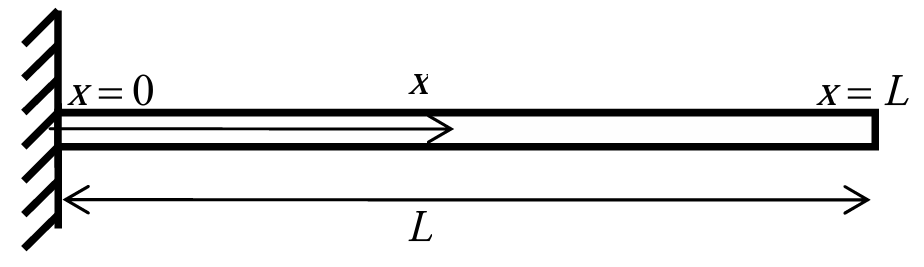
\includegraphics[width=0.5\linewidth]{figs/q48 49.png}
    \caption{}
    \label{fig:q48 49}
\end{figure}

\item To solve the PDE, the number of boundary conditions (BC) and initial conditions (IC) needed are
\begin{multicols}{4}
\begin{enumerate}
\item 4 BC, 3 IC
\item 2 BC, 2 IC
\item 2 BC, 4 IC
\item 4 BC, 2 IC
\end{enumerate}
\end{multicols}

\item For a cantilever beam, which of the following \textbf{CANNOT} be a possible boundary condition?
\begin{multicols}{4}
\begin{enumerate}
\item $w(0,t)=0$
\item $\frac{\partial^2 w}{\partial x^2}(L,t)=0$
\item $\frac{\partial^2 w}{\partial x^2}(0,t)=0$
\item $\frac{\partial^3 w}{\partial x^3}(L,t)=0$
\end{enumerate}
\end{multicols}

\textbf{Common Data questions 50 and 51}\\

Consider an inviscid, adiabatic flow of air at free stream Mach number $M_\infty=2$, across a compression corner ($\theta=20\degree$). The free stream total enthalpy is $h_{0\infty}=810$ kJ/kg. Assume that air is calorically perfect wit $\gamma = 1.4, R = 287\ J kg^{-1}K^{-1}$.

\item The shock angle $\beta$ is
\begin{multicols}{4}
\begin{enumerate}
\item $= 20\degree$
\item $> 20\degree$ and $< 30\degree$
\item $= 30\degree$
\item $> 30\degree$
\end{enumerate}
\end{multicols}

\item The total temperature at point $P$ is
\begin{multicols}{4}
\begin{enumerate}
\item $806.37$ K
\item $1128.92$ K
\item $1612.74$ K
\item $2257.84$ K
\end{enumerate}
\end{multicols}

\textbf{Linked Answer Questions}\\

\textbf{Statement for Linked Answer Questions 52 and 53:}\\

A thin-walled (thickness $<<$ radius), hollow shaft of length 1m and mean radius, $R = 5$ cm has to be designed such that it can transmit a torque, $T = 7$ kN-m. A survey of different commercially available materials was made and following data was obtained from the suppliers (E: Young’s modulus, $\tau_y$: yield stress in shear, $\rho$: density):
\begin{figure}[H]
    \centering
    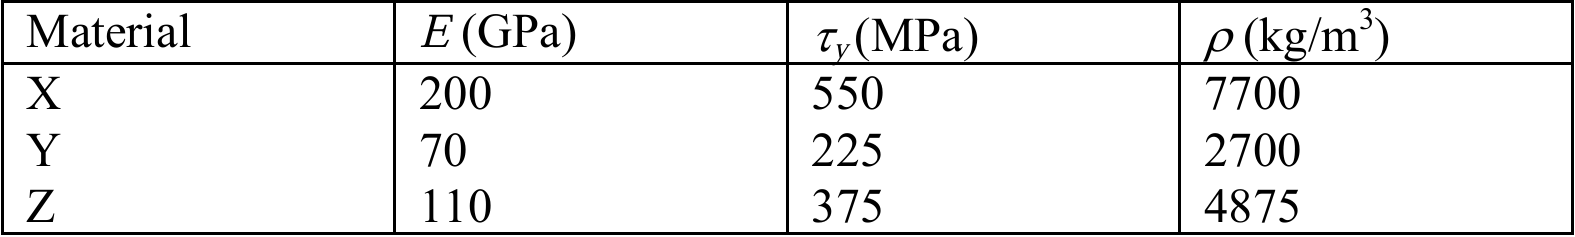
\includegraphics[width=0.5\linewidth]{tables/q52 53.png}
    \caption{}
    \label{fig:q52 53}
\end{figure}

\item Which of the above materials would you choose such that weight of the shaft is minimum? 
 \begin{multicols}{4}
    \begin{enumerate}        
        \item X only 
        \item Y only 
        \item Z only 
        \item X or Y
    \end{enumerate}
 \end{multicols}

 \item If you assume a factor of safety of 2, what should be the approximate thickness of such a shaft?
 \begin{multicols}{4}
    \begin{enumerate}    
    \item $0.5$ mm
    \item $1$ mm 
    \item $2$ mm 
    \item $4$ mm
    \end{enumerate}
 \end{multicols}

 \textbf{Statement for Linked Answer Questions 54 and 55:}\\

  
Prandtl’s lifting line equation for a general wing is given by 
$\alpha(y_\circ) = \frac{\Gamma(y_\circ)}{\pi U_{\infty} c(y_\circ)} + \alpha_{L=0}(y_\circ) + \frac{1}{4\pi U_\infty} \int_{\frac{-b}{2}}^{\frac{b}{2}}\frac{(\delta \Gamma/\delta y)}{y_\circ - y} dy$, where $U_\infty$ is the free-stream velocity, $\alpha$ is the 
angle of attack,  $\Gamma_\alpha=\frac{\partial \Gamma}{\partial \alpha}$ is the angle of attack, $y_\circ$ is the spanwise location, $\alpha_{L=0}(y_\circ)$ gives the spanwise variation of zero-lift angle, c is the chord, b is the span, and $\Gamma (y_\circ)$ gives the spanwise variation of circulation.

\item The rate of change of circulation with angle of attack $\Gamma_\alpha = \frac{\delta \Gamma}{\delta \alpha}$ is
\begin{multicols}{2}
\begin{enumerate}
\item inversely proportional to $\alpha$
\item independent of $\alpha$
\item a linear function of $\alpha$
\item a quadratic function of $\alpha$
\end{enumerate}
\end{multicols}

\item Given that $C_L \propto \int_{-b/2}^{b/2}\Gamma(y)\,dy$, the corresponding lift curve-slope $\frac{\partial C_L}{\partial \alpha}$ is
\begin{multicols}{2}
\begin{enumerate}
\item independent of $\alpha$
\item a linear function of $\alpha$
\item a quadratic function of $\alpha$
\item a cubic function of $\alpha$
\end{enumerate}
\end{multicols}


\textbf{General Aptitude (GA) Questions}\\

\textbf{Q.56 - Q.60 carry one mark each.}


\item Choose the word from the options given below that is most nearly opposite in meaning to the given word: \textbf{Deference}
\begin{enumerate}
\item aversion
\item resignation
\item suspicion
\item contempt
\end{enumerate}

\item Choose the most appropriate word(s) to complete the sentence: \textbf{We lost confidence in him because he never \underline{\hspace{2cm}} the grandiose promises he had made.}
\begin{enumerate}
\item delivered
\item delivered on
\item forgot
\item reneged on
\end{enumerate}

\item Choose the word or phrase that best completes the sentence: \underline{\hspace{2.5cm}} \textbf{in the frozen wastes of Arctic takes special equipment.}
\begin{enumerate}
\item To survive
\item Surviving
\item Survival
\item That survival
\end{enumerate}

\item In how many ways 3 scholarships can be awarded to 4 applicants, when each applicant can receive any number of scholarships?
\begin{multicols}{4}
\begin{enumerate}
\item 4
\item 12
\item 64
\item 81
\end{enumerate}
\end{multicols}

\item Choose the most appropriate word to complete the sentence: \textbf{The \underline{\hspace{2cm}} of evidence was on the side of the plaintiff since all but one witness testified that his story was correct.}
\begin{enumerate}
\item paucity
\item propensity
\item preponderance
\item accuracy
\end{enumerate}

\textbf{Q. 61 to Q. 65 carry two marks each.}\\

\item If $(2y+1)/(y+2) < 1$, which alternative gives the \textbf{CORRECT} range of $y$?
\begin{multicols}{4}
\begin{enumerate}
\item $-2<y<2$
\item $-2<y<1$
\item $-3<y<1$
\item $-4<y<1$
\end{enumerate}
\end{multicols}

\item A student attempted to solve a quadratic equation in $x$ twice. In the first attempt he incorrectly wrote the constant term and got roots $(4,3)$. In the second attempt he incorrectly wrote the coefficient of $x$ and got roots $(3,2)$. The roots of the correct quadratic equation are
\begin{multicols}{4}
\begin{enumerate}
\item $(-3,4)$
\item $(3,-4)$
\item $(6,1)$
\item $(4,2)$
\end{enumerate}
\end{multicols}

\item $L, M$ and $N$ are waiting in a queue meant for children to enter the zoo. There are 5 children between $L$ and $M$, and 8 children between $M$ and $N$. If there are 3 children ahead of $N$ and 21 children behind $L$, then what is the minimum number of children in the queue?
\begin{multicols}{4}
\begin{enumerate}
\item $28$
\item $27$
\item $41$
\item $40$
\end{enumerate}
\end{multicols}

\item Four archers $P, Q, R$ and $S$ try to hit a bull’s eye during a tournament consisting of seven rounds. As illustrated, a player receives 10 points for the bull’s eye, 5 points for the inner circle and 1 point for the outer circle.
\begin{figure}[H]
    \centering
    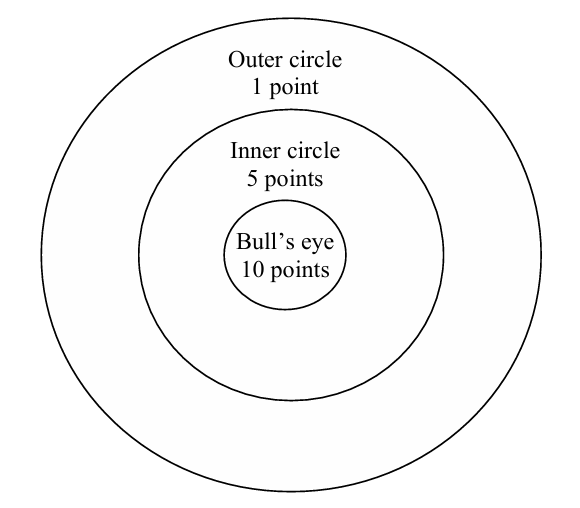
\includegraphics[width=0.5\linewidth]{figs/q64(1).png}
    \caption{}
    \label{fig:q64(1)}
\end{figure}
The final scores received by the players during the tournament are listed in the table below.
\begin{figure}[H]
    \centering
    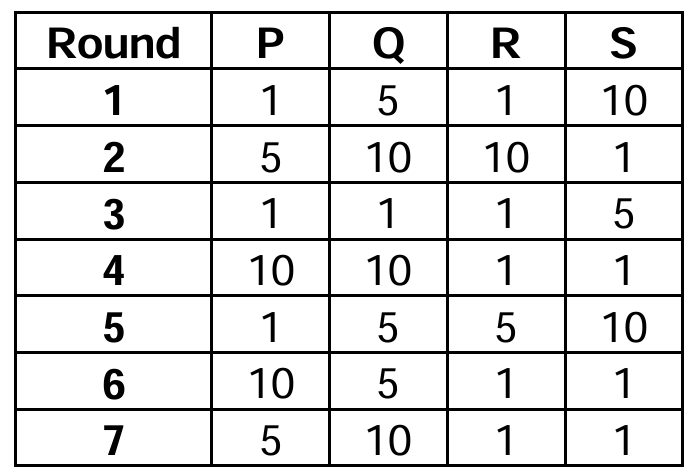
\includegraphics[width=0.3\linewidth]{tables/q64(2).png}
    \caption{}
    \label{fig:q64(2)}
\end{figure}
The most accurate and the most consistent players during the tournament are respectively
\begin{multicols}{4}
\begin{enumerate}
\item P and S
\item Q and R
\item Q and Q
\item R and Q
\end{enumerate}
\end{multicols}

\item \textbf{Nimbus clouds are dark and ragged, stratus clouds appear dull and cover the entire sky. Cirrus clouds are thin and delicate, whereas cumulus clouds look like cotton balls.}\\

It can be inferred that
\begin{enumerate}
\item A cumulus cloud on the ground is called fog
\item It is easy to predict the weather by studying clouds
\item Clouds are generally of very different shapes, sizes and mass
\item There are four basic cloud types: stratus, nimbus, cumulus and cirrus
\end{enumerate}

\end{enumerate}
\vspace{1cm}
\centering
\large
\textbf{END OF THE QUESTION PAPER}

\end{document}
